%
% $Id: icf.tex 14 2014-02-04 22:36:30Z nicb $
%
% p.77 cap.4 n.8
%
\svnInfo $Id: icf.tex 14 2014-02-04 22:36:30Z nicb $

\section{Introduzione\label{sec:icf introduction}}

I filtri comb inversi sono un caso particolare di filtri FIR. Essi permettono,
ad esempio, di cancellare le componenti di un segnale armonico.

Si tratta come sempre di un filtro FIR come quello studiato in
Sez.\ref{sec:simple fir}.\vref{sec:continuous time}  (eq.\ref{eqn:fir
semplice}). Sostituiamo al posto del ritardo arbitrario $\tau$ un numero
intero di campioni $L$. Come coefficiente del filtro prenderemo $R^{L}$.

L'equazione diventer\`a quindi

\begin{equation}\label{eqn:icf 1}
		y_t = x_t - R^{L} x_{t - L}
\end{equation}

e la sua funzione di trasferimento si ricaver\`a cos\`i

\begin{equation}\label{eqn: icf 1 tf}
  \begin{array}{r c l c c l}
	Y & = & 1 \times X z^{-0} - R^{L} \times X z^{-L} & = & X & \left [ 1 - R^{L} z^{-L} \right ]\\ 
	H ( z ) & = &                                     &   &   & \left [ 1 - R^{L} z^{-L} \right ]\\
	\end{array}
\end{equation}

\begin{quote}
Ripassiamo un p\`o di algebra dei numeri complessi.
Quali sono le radici dell'equazione seguente:

\begin{equation}\label{eqn: icf roots}
      z^{L} = 1
\end{equation}

Il teorema fondamentale dell'algebra dice che un polinomio di grado $n$ ha $n$
radici ($n$ punti in cui la funzione \`e zero). Prendiamo ad es.

\begin{equation}\label{eqn: tfa 1}
		y = x^{2} - 9
\end{equation}

Dobbiamo trovare i punti in cui $y = 0$. Allora:

\begin{equation}\label{eqn: tfa 2}
	\begin{array}{r c l}
		x^{2} - 9 & = & 0\\
		x^{2}     & = & 9\\
		x         & = & \sqrt{9}\\
		x         & = & \pm 3\\
	\end{array}
\end{equation}

% fare plot della funzione

E` possibile quindi pensare qualsiasi funzione nei termini delle sue radici:

\begin{equation}\label{eqn: tfa 3}
		y = a_1 ( x - r_1 ) (x - r_2) \dots
\end{equation}

P.es. nel caso dell'eq.\ref{eqn: tfa 2}

\begin{equation}\label{eqn: tfa 4}
	x^{2} - 9 = 1 ( x + 3 ) ( x - 3 )
\end{equation}

Spesso \`e necessario ricorrere ai numeri complessi per risolvere le
equazioni. P.es., quali sono le radici dell'eq.\ref{eqn: tfa complex 1}?

\begin{equation}\label{eqn: tfa complex 1}
	x^2 - x + 1 = 0
\end{equation}

Ricordando che

\begin{equation}\label{eqn: tfa complex 2}
				x = \frac{-b \pm \sqrt{b^{2} - 4 a c}}{2 a}
\end{equation}

e sostituendo i fattori $a$, $b$, e $c$ con quelli presenti nell'eq.\ref{eqn: tfa complex 1}

\begin{equation}\label{eqn: tfa complex 3}
				x = \frac{+1 \pm \sqrt{-1^{2} - 4 \times 1 \times 1}}{2 \times 1} = \frac{\pm \sqrt{1 - 4}}{2} = \frac{1}{2} \pm i \frac{\sqrt{3}}{2} = 0.5 \pm i 0.866
\end{equation}

In linea generale, le equazioni di grado $n$ con fattori complessi possiedono
$n$ radici in coppie complesse coniugate (per $n$ pari) oppure 1 radice reale
e $n - 1$ radici in coppie complesse coniugate (per $n$ dispari).
\end{quote}

Ecco dunque la risposta alla domanda: quali sono le radici dell'equazione $z^{L} = 1$?
ce ne sono $L$, complesse--coniugate e equispaziate sul cerchio
unitario. Questo \`e abbastanza ovvio quando si pensa a cosa significhi
innalzare un numero complesso alla sua $L$--esima potenza. Significa
elevare la sua magnitudine ($==$ il suo modulo) all'$L$--esima potenza e
moltiplicare il suo angolo per $L$. Qualsiasi punto con magnitudine 1 e
angolo in una forma $k 2 \pi / L$ funzioner\`a per qualsiasi $k$ intero.
Le $L$ radici dell'unit\`a saranno quindi:

\begin{equation}\label{eqn: roots of unity}
		e^{i k 2 \pi / L}~per~k = 0, 1, \dots, L - 1
\end{equation}

E nel caso dell'eq.\ref{eqn: icf 1 tf} le radici saranno:

\begin{equation}\label{eqn: roots of R}
		z^{L} = R^{L}
\end{equation}

e si troveranno agli stessi angoli, ma con raggio $R^{L}$ anzich\'e 1.

Facciamo un esempio con $L = 8$ (cio\`e: il segnale sar\`a composto
dall'ingresso pi\`u l'ingresso ritardato di otto campioni) con $R = 0.999999$.

Ci aspetteremo quindi di trovare otto zeri, e per la precisione (dato che il
segnale finale \`e reale) quattro coppie complesse coniugate.
In effetti, il plot sul piano zeta rappresentato in Fig.\vref{fig: icomb 8 zeroes}
mostra proprio che gli otto zeri si dispongono in maniera simmetrica intorno
all'asse reale (e anche simmetrica intorno all'asse immaginario).

\begin{figure}[htbp]
	\begin{center}
		\includegraphics[width=0.48\textwidth]{\plotdir/ICF2_2}
	  \includegraphics[width=0.48\textwidth]{\plotdir/ICF2_3}
		\caption{Disposizione degli zeri sul piano zeta per un filtro comb inverso di ordine 8\label{fig: icomb 8 zeroes}}
	\end{center}
\end{figure}

Come si pu\`o notare, gli zeri appaiono a $R^{L} e^{i 2 pi \times 0/L} = 1$,
$R^{L} e^{i 2 \pi \times 1/L} = R^{L} e^{i 2 \pi / 8} = R^{L} e^{i \pi / 4} = 0.707 + i 0.707$,
$R^{L} e^{i 2 \pi \times 2 /L} = R^{L} e^{i 4 \pi / 8} = e^{i \pi /2} = i$, ecc.
La Fig.\vref{fig: icomb 8 bode} invece mostra che la fase \`e per lo pi\`u
lineare, con gli shift di fase che accadono al passaggio dagli zeri della
magnitudine.

\begin{figure}[htbp]
	\begin{center}
	  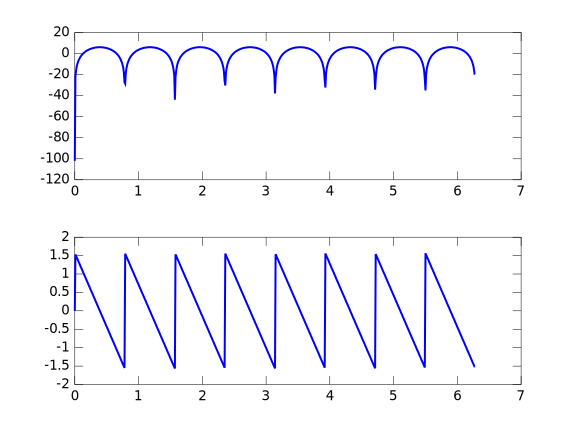
\includegraphics[width=0.8\textwidth]{\plotdir/ICF2_1}
	  \caption{Risposta in frequenza e in fase di un filtro comb inverso di ordine 8\label{fig: icomb 8 bode}}
	\end{center}
\end{figure}

\needspace{20\baselineskip}
Lo script \emph{octave} che produce questi plot \`e riportato qui di seguito:
\verbatiminput{\plotdir/ICF2.m}

Attenzione: un errore comune \`e quello di invertire l'ordine dei coefficienti nel
passare l'argomento alla funzione {\tt roots()} di \emph{matlab/octave}.
L'ordine \`e \ul{dal coefficiente pi\`u alto a quello pi\`u basso} (zero
incluso).

% esempio di signal cancellation
